%%%%%%%%%%%%%%%%%%%%%%%%%%%%%%%%%%%%%%%%%%%%%%%%%%%%%%%%
%
% Change the option between square brackets
% depending on the document you have to write:
%
% proposal    for the initial proposal
% review      for the literature review
% progress    for the progress report
% final       for the final report
% 
%%%%%%%%%%%%%%%%%%%%%%%%%%%%%%%%%%%%%%%%%%%%%%%%%%%%%%%%

\documentclass[progress]{cmpreport}
\makeatletter
\input{t1pcr.fd}
\makeatother
\setlength{\footnotesep}{3ex}
\usepackage{listings}
\usepackage{pgfplots}
% Some package I am using. You may not need them
%
\usepackage{rotating}
\usepackage{subfloat}

% packages for algorithms
\usepackage{amsmath}
\usepackage{algorithm}
\usepackage[noend]{algpseudocode}




%\setkeys{Gin}{draft}

%%%%%%%%%%%%%%%%%%%%%%%%%%%%%%%%%%%%%%%%%%%%%%%%%%%%%%%%
%
%  Fill in the fields with:
%
%  your project title
%  your name
%  your registration number
%  your supervisor's name
%
%%%%%%%%%%%%%%%%%%%%%%%%%%%%%%%%%%%%%%%%%%%%%%%%%%%%%%%%
\title{Progress Report- Investigating The Use Of Intelligent Search In AI For Solving Problems Efficiently}

%%%%%%%%%%%%%%%%%%%%%%%%%%%%%%%%%%%%%%%%%%%%%%%%%%%%%%%%
%
% The author's name is ignored if the following command 
% is not present in the document
%
% Before submitting a PDF of your final report to the 
% project database you may comment out the command
% if you are worried about lack of anonimity.
%
%%%%%%%%%%%%%%%%%%%%%%%%%%%%%%%%%%%%%%%%%%%%%%%%%%%%%%%%
\author{Luke Garrigan}


\registration{100086495}
\supervisor{Dr Pierre Chardaire}
%%%%%%%%%%%%%%%%%%%%%%%%%%%%%%%%%%%%%%%%%%%%%%%%%%%%%%%%
%
% Fill in the field with your module code.
% this should be:
%
% for BIS            -> CMP-6012Y
% for BUSINESS STATS -> CMP-6028Y
% for other students -> CMP-6013Y
%
%%%%%%%%%%%%%%%%%%%%%%%%%%%%%%%%%%%%%%%%%%%%%%%%%%%%%%%%
\ccode{CMP-6012Y}


\summary{
This document explains how to use the class file \texttt{cmpreport.cls} to write your reports.
The class file has been designed to simplify your life; many things are done for you. As a consequence
some commands presented here are specific to the class file whether they are new commands or customized versions
of commonly known \LaTeX\ commands.
}

\acknowledgements{
This section is used to acknowledge whoever's support and contribution.
The command that introduces it is ignored in the project proposal, literature review and progress report. It is used in the
final report,  but  is not compulsory. If you do not
have an acknowledgements command in your preamble then there
won't be any acknowledgement section in the document produced. \emph{Abstract} and \emph{Acknowledgements} sections should fit on the same page. 
}

%%%%%%%%%%%%%%%%%%%%%%%%%%%%%%%%%%%%%%%%%%%%%%%%%%%%%%%%%%%%%%%%%%
%
% If you do not want a list of figures and a list of tables
% to appear after the table of content then uncomment this line 
%
% Note that the class file contains code to avoid
% producing an empty list section (e.g list of figures) if the 
% list is empty (i.e. no figure in document).
%
% The command also prevents inserting a list of figures or tables 
% anywhere else in the document
%
% Some supervisors think that a report should not contain these
% lists. Please ask your supervisor's opinion.
%
%%%%%%%%%%%%%%%%%%%%%%%%%%%%%%%%%%%%%%%%%%%%%%%%%%%%%%%%%%%%%%%%%%
%\nolist,

%%%%%%%%%%%%%%%%%%%%%%%%%%%%%%%%%%%%%%%%%%%%%%%%%%%%%%%%%%%%%%%%%%
%
% Comment out if you want your list of figures and list of
% tables on two or more pages, in particular if the lists do not fit 
% on a single page.
%
%%%%%%%%%%%%%%%%%%%%%%%%%%%%%%%%%%%%%%%%%%%%%%%%%%%%%%%%%%%%%%%%%%
\onePageLists

\begin{document}


\section{Introduction}
A classic example in the AI literature of pathfinding problems are the sliding-tiles puzzles such as the $3\times3$ Eight Puzzle, the $4\times4$ 15 puzzle and the $5\times5$ twenty-four puzzle. The Eight Puzzle consists of a $3\times3$ grid with 8 numbered square tiles and 1 blank. The blank is used to slide other tiles in which are horizontally or vertically adjacent into that position in an attempt to reach the goal state. The objective of the puzzle is to move the tiles from a set composition to a goal configuration, which is with the numbers in ascending order from 1 to 8.
The sliding-tile puzzle is exclusively targeted throughout the following literature. 

A search algorithm is a series of steps that can be used to find the location or the path of a desired state. In most scenarios there will be additional constraints that will need to be fulfilled such as the time taken to reach the desired state, memory availability, maximum number of moves.

 In this progress report the main focus was to implement and test algorithms for finding the goal state of the sliding tile puzzle in the minimum number of moves, with the prospect of scalability in mind. In doing so I'd sought out to find and identify the major flaws of varying search algorithms and seek methods to adhere to these pitfalls. 
 
\section{Program Architecture}
I have written depth-first search, breadth-first search, iterative deepening depth-first search and A* in a multitude of languages such as Prolog, PHP and Python, this paper however shows the findings of the search algorithms exclusively written in Java. 
\subsection{Initial Implementation}
Originally I deemed it wise to represent the states of the sliding tile puzzle as a two dimensional array as this way I would always know which row and column a given value was in and finding the possible moves from that point would be trivial:
\begin{verbatim}
	int[] goalState ={{1,2,3},{4,5,6},{7,8,0}};
\end{verbatim}
Continuously creating new two-dimensional arrays for neighbouring states became quite costly so I adapted the code to adhere to one dimension. 
\begin{verbatim}
int[] goalState ={1,2,3,4,5,6,7,8,0};
\end{verbatim}

The State class contains the array of the current configuration of the state which is used to compare against the  desired goal state. A Node object of it's parent is stored, which allows us to find the path taken to arrive at the goal node by looping through each Node until there are no more existing parents thus having reached the initial node. The direction is stored to be outputted when the goal Node is found.     

\begin{verbatim}
public State(int moves, byte[] composition, int zeroPosition) {
    this.moves = moves;
    this.composition = composition;
    this.zeroPosition = zeroPosition;
}

\end{verbatim}
When a node is being expanded it is necessary to find its neighbours. Neighbours for the sliding-tile puzzle represent the possible moves from the current configuration, each state has a minimum of 2 neighbours and a maximum of 4. Figure 1 shows the possible moves from current state and how the direction variable would be stored ready for output. 

\begin{figure}[ht]
	\centering
	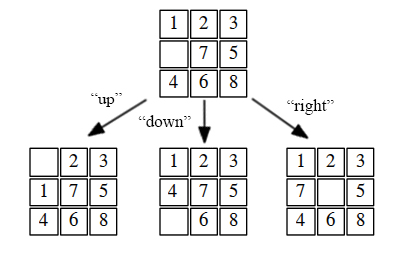
\includegraphics[width=0.5\textwidth]{moves}
	\captionsetup{justification=centering}
	\caption{Finding possible moves}
\end{figure}


\section{Brute-Force Search}
Brute-force search is a general problem-solving technique that consists of systematically enumerating all the possible options for a given solution and checking to see whether that given option satisfies the problem's statement. All that is required to execute a brute-force is some legal operators, an initial state and an acknowledged goal state. 

\subsection{Breadth-First Search}
Breadth-first search expands the nodes in a tree in the order of their given distance from the root, so it expands all the neighbouring nodes before going to the next level of the tree. Because the algorithm doesn't trawl to the deeper levels of the tree without first expanding the lower levels, it ensures the finding of the shortest path. The amount of time used by breadth-first search is linear to the number of nodes expanded, since each node can be generated in constant time, and is a function of the branching factor $b$ and the solution depth $d$. Since the number of nodes at level $d$ is $b^d$, the total number of nodes generated in the worst case is $O(b^d)$. \citep{DBLP:journals/mima/Korf95}.

The initial algorithm I implemented to solve the 8-tile puzzle was the breadth-first search as it guarantees to find the solution in minimal steps. The space requirement of breadth-first search is it's largest deficiency. The 8-tile has a search space of $9!/2=181,400$ with a maximum number of 31 moves to solve. In terms of practicality, with larger problem states such as the 15-tile puzzle a breadth-first search will exhaust the available memory rather quickly with its $16!/2 = 10,461,394,944,000$ search space and a maximum number of 80 moves to solve.

Table 1 shows the results of the breadth-first search algorithm in the 8-tile puzzle. The algorithm was tested on states of varying complexity from a minimum of 5 moves to solve, to  a minimum of 20. As established, breadth-first search finds the optimal solution to a goal state with the minimum number of moves. As the difficulty of the initial puzzle state increases the number of nodes expanded increases exponentially along with the time taken. This proves the previously stated theory that the number of nodes generated in the worst case is $O(b^d)$.


\begin{table}[ht]
	\caption{Breadth-First Search Analysis: 8-Tile}
	\begin{center}
		\begin{tabular}{crrr} \hline
			Min Moves & Moves & Nodes Expanded &Time(ms)  \\ \hline
			5  & 5 & 60& 2.097152 \\
			10 & 10 &619&  10.48576 \\ 
		    15 & 15 & 8159& 448.79053 \\ 
	    	20 & 20& 65638 & 34621.883 \\ \hline
		\end{tabular}
	\end{center}
\end{table}



\subsection{Depth-First Search}
Depth-first search (DFS) addresses the limitations of breadth-first by always generating next a child of the deepest unexpanded node. Breadth-first search manages the list as a first-in first-out queue, whereas depth-first search treats the list as a last-in first-out stack. Depth-first search is implemented recursively, with the recursion stack taking the place of an explicit node stack. Given a starting state, depth-first search stores all the unvisited children of that state in a stack. It then removes the top state from the stack and adds all of the removed states children to the stack. Depth first search generates a long sequence of moves, only ever reconsidering a move when it reaches the end of a stack, this can become a serious problem given a graph of significant size and there's only one solution, as it may end up exploring the entire graph on a single DFS path only to find the solution after looking at each node. Worse, if the graph is infinite the search might not terminate.



Depth-first search is not the preferred algorithm for solving the sliding-tile puzzle especially with the goal of solving the puzzle in the minimum number of moves, it would be more preferred in an implementation which has goals in every path. I decided to implement the algorithm regardless to analyse whether the results match expectation. Table 2 displays the results of the depth-first search implementation, there is no real noticeable pattern in the data apart from they are consistently inconsistent. The results prove that the algorithm doesn't find the goal state in the minimum number of moves which further confirms that DFS should not be used in the sliding-tile problem. 

\begin{table}[ht]
	\caption{Depth-First Search Analysis: 8-Tile}
	\begin{center}
		\begin{tabular}{crrr} \hline
			Min Moves & Moves & Nodes Expanded &Time(ms)  \\ \hline
			5  & 57510 & 112377 & 352451.56 \\
			10 & 7817 &8199&  1021.31305 \\ 
			15 & 61050 & 94710& 273506.38 \\ 
			20 & 21123& 22420 & 11370.758 \\ \hline
		\end{tabular}
	\end{center}
\end{table}

  
\subsection{Depth-First Search Iterative Deepening}
Depth-First Iterative-Deepening (DFID) is an extension of depth-first search, it combines breadth-first search's completeness and depth-first search's space efficiency. DFID has a maximum depth, so it searches all possibilities up to a certain depth and if it doesn't find the goal state it increases the search depth. DFID performs depth-first search to depth one, then starts over and executes a depth-first search to depth two and continues deeper and deeper until a solution is found. The complexity of DFID is only O(d) where d is the depth, this is because at a given point it is executing only a depth-first search and saving only a stack of nodes. DFID ensures that the shortest path to the goal state will be found as does breadth-first search. \citep{DBLP:conf/otm/MeissnerB11}.
\makeatletter
\def\BState{\State\hskip-\ALG@thistlm}
\makeatother

\begin{algorithm}
	\caption{My algorithm}\label{euclid}
	\begin{algorithmic}[1]
		\Procedure{MyProcedure}{}
		\State $\textit{stringlen} \gets \text{length of }\textit{string}$
		\State $i \gets \textit{patlen}$
		\BState \emph{top}:
		\If {$i > \textit{stringlen}$} \Return false
		\EndIf
		\State $j \gets \textit{patlen}$
		\BState \emph{loop}:
		\If {$\textit{string}(i) = \textit{path}(j)$}
		\State $j \gets j-1$.
		\State $i \gets i-1$.
		\State \textbf{goto} \emph{loop}.
		\State \textbf{close};
		\EndIf
		\State $i \gets i+\max(\textit{delta}_1(\textit{string}(i)),\textit{delta}_2(j))$.
		\State \textbf{goto} \emph{top}.
		\EndProcedure
	\end{algorithmic}
\end{algorithm}



\begin{verbatim}	
public void IDDFS(State root) {
// Keep on looping until a goal state is found
    for (int depth = 0; depth < Integer.MAX_VALUE; depth++) {
        State found = DLS(root, depth);
        if (found != null) {
            System.out.println("Goal found");
        }
    }
}
public State DLS(State node, int depth) {
    if (depth == 0 && Arrays.equals(node.getState(), GOAL)) {
        return node;
    }
    if (depth > 0) {
        // finds the neighbours then loops through each
        // and performs the limited search on each neighbour
        for (State neighbour : node.findNeighbours()) {
            State found = DLS(neighbour, depth - 1);
            if (found != null) {
                System.out.println(Arrays.toString(found.getState()));
                return found;
            }
        }
    }
    return null
\end{verbatim}

Although DFID maintains the advantage of requiring a comparable supply of memory as depth-first search and doesn't get caught in infinite loops, DFID's time taken to find a solution is vast and generally longer than both depth-first search and breadth-first search, this is because it has to expand the same states multiple times. Table 3 are the results for DFID with the depth preset to the minimum number of moves required to solve the puzzle state. It is clear that the number of nodes expanded is far greater in comparison with breadth-first search shown in Table 1.

\begin{table}[ht]
	\caption{Depth-First Iterative Deepening: 8-Tile}
	\begin{center}
		\begin{tabular}{crrr} \hline
			Min Moves & Moves & Nodes Expanded &Time(ms)  \\ \hline
			5  & 5 & 56 & 0.9521 \\
			10 & 10  &6392&  16.777216 \\ 
			15 & 15 & 3350884& 2902.4583  \\ \hline
		
		\end{tabular}
	\end{center}
\end{table}



\subsection{Evaluation Of Brute-Force Searches}
Depth-first search often provokes the possibility of going down the left-most path forever, it is also not guaranteed to find the solution and the likelihood that the solution found is optimal is unlikely, so for the sliding-tile puzzle in general this is not useful. 

Breadth-first search is relatively fast when considering the 8-tile puzzle as the search space is small, however it uses too much memory to be useful with larger problems such as the 15-tile puzzle. 

Depth-first iterative deepening is beneficial as it avoids infinite cycling, it obtains the same result as BFS whilst saving memory, however it is very slow as it has to repeatedly expand nodes it has already visited. DFID is only really beneficial when the solution depth is known, else it would have to trawl through all possibilities up to the solution depth and then through all possibilities at the solution depth until it reaches the goal. It is unlikely for the sliding-tile puzzle that the user knows the solution depth, thus implies ample execution time to find the goal state.


\section{Heuristic Search} \label{sec1}
In order to improve the search efficiency I decided to adopt some heuristic functions. A heuristic is a method that might not always find the best solution but it will guarantee to find a good solution in a reasonable time. The idea behind a heuristic function is that it sacrifices the completeness in order to increase efficiency. They are usually utilised in solutions in which may take infinite time or a very long time to compute. \citep{DBLP:conf/ai/2014}. 


\subsection{Admissible Heuristics}
A heuristic function is said to be admissible if it never overestimates the cost of reaching the goal, i.e the estimated cost to the goal from the current node is not higher than the lowest possible cost from the current node. The lowest possible cost $h^*(n)$ is the cost of the optimal path from $n$ to a goal node $G$. The heuristic function $h(n)$ is admissible if $0 \leq h(n) \leq h^*(n)$, essentially meaning admissible heuristic functions are optimistic.

\subsection{Consistent Heuristics}
One crucial characteristic of the heuristic required for my analysis is that it must be consistent. A heuristic function is said to be consistent if the cost from the current node $n$ to a successor node $p$, plus the estimated cost from the successor node to the goal state is less than or equal to the estimated cost from the current node to the goal node $h(n)\leq c(n,p) + h(p)$, where $c(n,p)$ is the cost of reaching node $p$ from $n$ and the heuristic value of the goal $G$ is zero $h(G)=0$. 


\begin{figure}[ht]
	\centering
	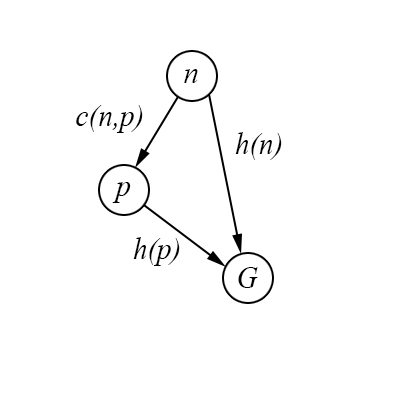
\includegraphics[width=0.4\textwidth]{consistent}
	\captionsetup{justification=centering}
	\caption{Consistent Heuristics Diagram}
\end{figure}



 

Heuristic search allowed me to find faster solutions to the sliding-tile puzzle and even gave me the opportunity to increase the search space, so moving up to the 15-tile puzzle.

\subsection{Heuristic Evaluation Functions}
\subsubsection{Manhattan Distance}
A common heuristic function for the sliding-tile puzzle is called Manhattan distance. The Manhattan distance is the distance between two points in a grid, based on a strictly horizontal and/or vertical path and summing these values over all tiles. For a fixed goal state, a heuristic evaluation is a function of a node, $h(n)$ in which estimates the distance from the node to said goal state.


Heuristic evaluation functions estimate the actual cost with very little computational power, thus very compelling. The complexity of the Manhattan Distance is proportional to the number of tiles between the initial state and the goal state. Most heuristic functions are lower bounds on the actual cost deeming them admissible. The Manhattan distance is a lower bound for the number of moves required to solve an occurrence of the sliding-tile puzzle, since every tile must move at least as many times as its distance to its goal position. \citep{DBLP:conf/ccgrid/LinnertSB14}.

\begin{verbatim}
public int manhattan(int[] puzz) {
int total = 0;
for (int i = 1; i < puzz.length; i++) {
    int expectedRow = (i - 1) / 3;
    int expectedCol = (i - 1) % 3;
    int num = 0;
        for (int j = 0; j < puzz.length; j++) {
            if (puzz[j] == i) {
            num = j + 1;
            break;
        }    
    }
    int numRow = (num - 1) / 3;
    int numCol = (num - 1) % 3;
    total += Math.abs(expectedRow - numRow)
    + Math.abs(expectedCol - numCol);
    }
    return total;
}
\end{verbatim}
\subsubsection{Linear Conflict Heuristic}
Linear Conflict is somewhat similar to Manhattan distance in regards to the sum of the displacement of each each tile, however it also recognises that given two tiles which are both correctly placed in their desired row/column but they are in the wrong order, one of these tiles will have to move out of the row/column in order to let the other pass. If there is a linear conflict then an extra two moves will be added to the total sum as the tile which must move, has to transition out of the row/column and then back into it's desired position.

 
\begin{verbatim}
private int linearVerticalConflict(int[] state) {
    int dimension = 3;
    int linearConflict = 0;
    int count =0;
    for (int row = 0; row < dimension; row++) {
        int max = -1;
        for (int column = 0; column < dimension; column++) {
            int cellValue = state[count];
            count++;
            if (cellValue != 0 && (cellValue - 1) /
             dimension == row) {
                if (cellValue > max) {
                   max = cellValue;
                } else {
                    linearConflict += 2;
                }
            }
        }
    }
    return linearConflict;
}
\end{verbatim}

Above is the code I wrote in order to calculate the linear conflict of the rows, I then took the sum of the linear conflict of this and the columns as the total heuristic value for the given state. The algorithm loops through the columns and the rows, finding the value and checks whether it is in it's goal row. If it is in it's goal row it then checks whether it is greater than the current maximum because if it is not then the previous value is greater, thus they are in the wrong order; as the sliding tile goal state is ascending. 

Figure 2 displays a visual example of how the linear conflict is working. The initial state shows the first row to be reversed meaning values 1,2 and 3 are positioned 3,2 and 1. When looping through the values the $max$ is compared to 3, as 3 is greater than -1 $max$ is now 3. For value 2 it is not larger than the current $max$ 3 so a linear conflict has happened thus 2 is added to the total, value 1 is also not larger than 3 thus another two is added to the total heuristic value.


\begin{figure}[ht]
	\centering
	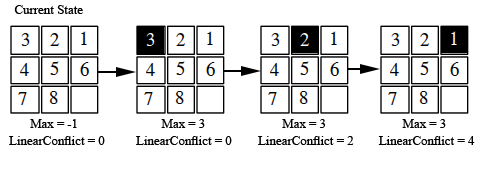
\includegraphics[width=0.9\textwidth]{linear}
	\captionsetup{justification=centering}
	\caption{Calculating Linear Conflict}
\end{figure}



\subsection{A* Algorithm}
A* search is a combination of lowest-cost-first and best-first searches that considers both path cost and heuristic information in its selection of which path to expand. For each path on the frontier, A* uses an heuristic of the path cost from a start node to a goal node constrained to start along that path. This allows A* search to ensure the prioritisation of states in which are more likely to result in a low-cost goal state. The calculation of the heuristic value is dependent on the problem that is being solved. For example, for problems which aim to reach a location the Euclidean distance between the state and the goal is often used as the heuristic. 

The A* algorithm uses $cost(p)$, the cost of the path found, as well as the heuristic function $h(p)$, the estimated path cost from the end of $p$ to the goal. As A* uses admissible heuristic it will always find solutions in the order of their cost. \citep{DBLP:journals/ker/Brewka96}.  A* uses breadth-first traversal thus uses large chunks of memory in comparison to applications that use depth-first traversal. The performance of A* is also heavily reliant on the accuracy of the heuristic.

\begin{verbatim}
OPENSET.add(initialState);
while (OPENSET.isEmpty() == false) {
    if (OPENSET.size() > 0) {
        int winner = 0;
        for (int i = 0; i < OPENSET.size(); i++) {
            if (OPENSET.get(i).getF() < OPENSET.get(winner).getF()) {
            winner = i;
            }
        }
        State currentState = OPENSET.get(winner);
        if (Arrays.equals(currentState.getState(), GOAL)) {
            printPath(currentState, startTime); // prints out path and time taken
            break;
        }
        OPENSET.remove(currentState);
        CLOSEDSET.add(currentState);
        ArrayList<State> neighbours =  currentState.findNeighbours();;
        for (int i = 0; i < neighbours.size(); i++) {
            State neighbour = neighbours.get(i);
            if (!CLOSEDSET.contains(neighbour)) {
                float tempG = currentState.getG() + 1;
                if (OPENSET.contains(neighbour)) {
                    if (tempG < neighbour.getG()) {
                        neighbour.setG(tempG);
                    }
                } else {
                   neighbour.setG(tempG);
                   OPENSET.add(neighbour);
                }
                int man = manhattan(neighbour.getState());
                neighbour.setH(man);
                neighbour.setF(neighbour.getG() + neighbour.getH());
           }
       }
  }
\end{verbatim}

The implementation I made for the A* algorithm works by initially declaring an empty $OPENSET$ and an empty $CLOSEDSET$ which are both  $ArrayList$s of the $State$ object. The commencing $State$ is added to the $OPENSET$, the $OPENSET$ is then looped through to find the $State$ with the smallest $F$ value, which is assigned to the $winner$ variable. The $currentState$ is then assigned to the State which contains that smallest $F$ value, this is then checked against the $GOAL$ state to check whether it is the solution. If it isn't a goal state it is removed from the $OPENSET$ and added to the $CLOSEDSET$ because we don't want to expand the same $State$ again.
The neighbours for the $currentState$ are then found and looped through. If the neighbour is not in the $CLOSEDSET$ it hasn't been expanded, the $G$ value is assigned to the neighbour which is just the $currentStates$'s $G+1$, as in the sliding tile puzzle a tile can only move one position at a time. It then checks whether the neighbour is in the $OPENSET$ as there's a chance we got to this neighbour more optimally than the previous path, if so it reassigns the values. The $F$ value is then calculated for the neighbour by adding the $G$ and the $H$ value, the program then repeats the process.


\subsubsection{Linear Conflict Or Manhattan Distance}
My tests displayed in Table 4 show that A* search with the linear conflict heuristic improves the performance of A* with Manhattan distance for the 8-tile puzzle. On average A* with linear conflict would take around 1ms longer than A* with Manhattan distance, until the number of moves required to solve the puzzle were greater than 25, as this showed a substantial decline in time when comparing the linear conflict to the Manhattan heuristic. This implies that the performance of linear conflict exceeds the performance of Manhattan distance when the state space grows, so the more difficult the puzzle the greater the gap in performance between the two heuristics becomes.
\begin{center}
	\captionof{table}{Manhattan Distance Vs. Linear Conflict - A*}
	\begin{tabular}{|l|r|r|r|r|r|r|} \cline{2-7}
		
		\multicolumn{1}{c}{} & \multicolumn{3}{|c|}{Manhattan Distance} &
		\multicolumn{3}{|c|}{Linear Conflict} \\ \hline
		Min Moves & Time(ms) & Mean Memory & States & Time(ms) & Mean Memory & States \\	\hline \hline
		5 & 0.3170 & 4.0267 & 6               & 1.3602 & 4.0267 & 6 \\
		10 & 0.4326 & 4.0267 & 11             & 1.3391 & 4.0267 & 11 \\
		15 & 0.5599 & 4.0267 & 16             & 1.4346 & 4.0267 & 16 \\
		20 & 0.7307 & 4.0267 & 21             & 1.6672 & 4.0267 & 21 \\
		25 & 4.4329 & 4.0267 & 141            & 4.2708 & 4.0267 & 103\\
		30 & 532.9964 & 4.9195 & 5640         & 277.7063& 5.3643 &3752\\
		\hline
	
	\end{tabular}

\end{center}
 As the state space grows exponentially according to the depth the growth is smaller for the A* with linear conflict, this is because the heuristic is a more accurate representation of the displacement of the tiles, thus the H value is always larger than or equal to the H value of the Manhattan Distance. Table 5 shows the difference in H value for 10 calculations of both algorithms and how the linear conflict is nearly always larger than the Manhattan distance.
 
  Table 4 shows the exponential growth by the number of states the algorithm expanded. The average number of States for the Manhattan distance heuristic from 5 to 30 moves is 972.5, whereas linear conflict's average is 651.


\begin{table}[ht]
	\caption{Manhattan Distance Vs Linear Conflict Values}
	\begin{center}
		\begin{tabular}{crr} \hline
			State & Manhattan Distance  & Linear Conflict    \\ \hline
			1  & 20 & 22  \\
			2 & 20  & 26 \\ 
			3 & 20 & 24  \\ 
			4 & 22 & 24  \\
		    5 & 21  & 23 \\ 
			6 & 21 & 23  \\ 
			7 & 21 & 23  \\ 
			8 & 21 & 23  \\ 
			9 & 22 & 22  \\ 
			10 & 20 & 22  \\ \hline
		\end{tabular}
	\end{center}
\end{table}


\section{Fifteen Tile Puzzle}
I initially tested the A* Manhattan distance and the A* linear conflict on the fifteen tile puzzle, however could only get results for puzzle states which require a small number of moves to find the goal. The reasoning for the lack of results is the large amount of States that the $CLOSEDSET$ has to store. 

A* uses breadth-first traversal thus the number of states that are stored increases exponentially with depth. I needed to find an algorithm which would require less memory but still have the benefits of a heuristic search. This is similar to the previous scenario when considering how to reduce the memory used in breadth-first by taking depth-first search's memory used as inspiration.

The memory used by Depth-first iterative deepening is linear with respect to the depth. In theory DFID could be used to solve the 15-puzzle without running out of memory, however taking the results found in Table 3, the time taken to reach the goal state for any random instance of the fifteen tile puzzle would be unreasonable.


\subsection{Iterative Deepening A*}
Iterative-deepening-A* (IDA*) eradicates the memory complication of A* by using depth-first traversal, without sacrificing solution optimality at the cost of increasing the time taken. Each iteration of A* is a complete depth-first search that keeps track of the cost, $f(n) = g(n) = h(n)$, of each node generated. If an expanded node's cost generated exceeds a threshold for that iteration, its path is cut off and the search backtracks before continuing. IDA* ranks states the same way as A*: The expected cost of a state is the cost of reaching said state and the heuristic's estimate of the cost of reaching the nearest goal state. The maximum expected cost is assigned to the heuristic cost of the starting state, states in which have a lowest cost than the starting state are traversed and states with a higher expected cost are discarded. 


If IDA* has searched all states lower than the current maximum without finding the goal state then it increases the maximum to the lowest value of the discarded states and begins the search again. The goal state is admissible, the current maximum cost will never be higher than the lowest cost solution, thus IDA* with an admissible heuristic will always find the lowest cost solution.  IDA* searches many nodes multiple times thus is slower than A*. Hence, A* should be used on smaller applications that aren't going to have memory issues.

\begin{verbatim}

public State IDAStar(State start) {
    nextCostBound = start.getH();
    State solution = null;
    while (solution == null) {
        float currentCostBound = nextCostBound;
        solution = depthFirstSearch(start, currentCostBound);
        nextCostBound += 2;
    }
    return solution;
}
public State depthFirstSearch(State current, float currentCostBound) {
    if (Arrays.equals(current.getState(), GOAL)) {
       return current;
    }
    for (State next : findNeighbours(current)) {
        next.setG(current.getG() + 1);
        float li = l.linearConflict(next.getState());
        next.setH(li);
        float value = next.getG() + next.getH();
        if (value <= currentCostBound) {
            State result = depthFirstSearch(next, currentCostBound);
            if (result != null) {
                return result;
            }
        }
    }
    return null;
}

\end{verbatim}

The Java implementation of the IDA* algorithm above begins by initially retrieving the $H$ value of the $start$ node as it has already been set during object creation. The code then loops through until a solution is returned from the $depthFirstSearch()$ method that isn't null, thus the goal node. The float $currentCostBound$ is assigned to $nextCostBound$ and used to perform the depth-first search to that threshold, the bound is increased each time. 

The $depthFirstSearch()$ initially checks whether the $current$ State is equal to the goal node and if so returns it, else it will then further loop through it's neighbours. Whilst looping, the $G$ value is set 
for the neighbours which is the number of moves taken to get there, so it is the parent's $G$ value incremented by one. The heuristic value is then calculated, in this case the linear conflict heuristic and then the sum of the $G$ and the $H$ form the $F$, which is used to determine which of the moves is the best from the $current$ State, and if the $F$ value is lower than the $currentCostBound$ then a recursive call on $depthFirstSearch$ method is called with the neighbour as the argument. 
\captionof{table}{Iterative Deepening A* Results}
\begin{center}

	\begin{tabular}{|l|r|r|r|r|} \cline{2-5}
		
		\multicolumn{1}{c}{} & \multicolumn{2}{|c|}{Linear Conflict} &
		\multicolumn{2}{|c|}{Manhattan Distance} \\ \hline
		Min Moves & Time(ms) & States Expanded & Time(ms) & States Expanded \\	\hline \hline
		5  & 2.2913 & 6                        & 2.4060       &          6            \\
		10 & 2.3751  & 13                      & 2.3739       &         11            \\
		15 & 2.8140 & 24                       & 2.5081          &      16            \\
		20 & 11.3692 & 919                     & 8.0932        &        768           \\
		25&  21.9585  & 10420                  & 37.5986        &       25272         \\
		30& 117.3271 & 91471                   & 159.5604        &      217239        \\
		35  & 215.4406 & 231508                & 287.0284        &      482893        \\
		40& 78.972869 & 61141                  & 120.4332          &    110903        \\
		45 & 1750.4441 & 2468006               & 7111.9494        &     14202684      \\
		50& 9162.8202 & 13704525               & 17143.5055         &   36202294       \\
		55 & 6233.2757 & 9132143               & 13912.0609        &    29537720       \\
		60 & 61771.3520 & 87466771             & 277232.1371      &     596363837      \\
		\hline
		
	\end{tabular}
	
\end{center}




\begin{figure}[!ht]
	
	\begin{subfigure}[t]{.5\textwidth}
		\begin{tikzpicture}
		\begin{axis}[
	 width=\textwidth,
	axis lines = left,
	xlabel = Min Moves,
		]
	\addplot coordinates{(5,2.5849)(10,3.7)(15,4.5849)(20,9.8439)(25,13.347)(30,16.481)(35,17.8207)(40,15.899)(45,21.234)(50,23.708)(55,23.122)(60,26.382217)};
	
	\addplot
	coordinates{(5,2.5849)(10,3.459)(15,4)(20,9.5849)(25,14.62626)(30,17.72892)(35,18.881)(40,16.7589)(45,23.7596)(50,25.10958)(55,24.81606)(60,29.15162)};
		
		\end{axis}
		\end{tikzpicture}
		\caption{Log Of The States Expanded}
	\end{subfigure}%
	\begin{subfigure}[t]{.5\textwidth}
		\begin{tikzpicture}
		\begin{axis}[
		width=\textwidth,
		axis lines = left,
		xlabel = Min Moves,
		]
	\addplot coordinates{(5,1.1961)(10,1.2479)(15,1.492622)(20,3.507059)(25,4.456708)(30,6.874392)(35,7.7511)(40,6.303)(45,10.773)(50,13.161)(55,12.60577)(60,15.91465)};
	
	\addplot
	coordinates{(5,1.2666)(10,1.2472)(15,1.3265)(20,3.01)(25,5.232)(30,7.31795)(35,8.16505)(40,6.912089)(45,12.79603)(50,14.0653)(55,13.76405)(60,18.08073)};
		\end{axis}
		\end{tikzpicture}
		\caption{Log Of The Time}
	\end{subfigure}
	\caption{Logarithmic Comparison Of IDA* Fifteen Tile}
\end{figure}

The time complexity of IDA* is measured by the number of nodes expanded, provided each node can be expanded and it's successors evaluated in constant time, the asymptotic time complexity of IDA* is the total nodes expanded. Otherwise it is the product of the total number of nodes and the time taken to expand each. Provided the heuristic is consistent (see 4.2), IDA* must expand all nodes with the $f$ value less than or equal to $c$ which  is the cost of an optimal solution $f(n) \leq c$. This is shown in my code by \begin{verbatim}
if(value <= currentCostBound)
\end{verbatim}

On the final iteration of IDA* the cost threshold is equal to $c$, the cost of an optimal solution.\citep{DBLP:journals/ai/KorfRE01}.

The results I gathered shown in Table 6 and Figure 4 further compliment the findings of the contrast in efficiency of the two heuristics Manhattan distance and Linear conflict. With the number of states expanded increasing the time taken to find the goal state increases and thus the difference between the linear conflict and Manhattan Distance widens.


\section{Pattern Databases}
\subsection{Solvability Of Tile Games}
Problem domains may have constraints that can preclude parts of the search space. For example, although the fifteen puzzle has $ 16! \approx 10^{13} $ possible positions, only one half of them can be reached from the goal. \citep{DBLP:journals/ci/CulbersonS98}. 

To determine whether a sliding-tile puzzle is solvable we must calculate the sum of the inversions.
An inversion is when a tile precedes another tile with a smaller number on it. The first step we need to take is to flatten the puzzle as shown in Figure 5, for my implementation the puzzle is already stored as an array.
There are 3 rules we must adhere to: \citep{WinNT}
\begin{itemize}
 	\item If the grid width is odd, then the number of inversions must be even.
	\item If the grid width is even, and the blank is on an even row counting from the bottom then the number of inversions must be odd.
	\item If the grid width is even, and the blank is on an odd row counting from the bottom then the number of inversions must be even. 
	
\end{itemize}




\begin{figure}[ht]
	\centering
	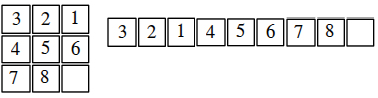
\includegraphics[width=0.6\textwidth]{parity}
	\captionsetup{justification=centering}
	\caption{Puzzle Parity}
\end{figure}

Here is some code I wrote to calculate the sum of the inversions in an array, from this we can determine whether it is solvable by following the guidelines above.
\begin{verbatim}
static int getInvCount(int arr[]) {
    int inv_count = 0;
    for (int i = 0; i < arr.length - 1; i++) {
        for (int j = i + 1; j < arr.length; j++) {
            if (arr[i] > arr[j]) {
                inv_count++;
            }
        }
   }
   return inv_count;
}
\end{verbatim}


\subsection{Non-Additive Pattern Databases}
A Pattern Database stores a collection of solutions to sub-problems that much be achieved to solve the overall problem. They are admissible heuristic functions implemented as lookup tables that store the lengths of optimal solutions for sub-problem instances. \citep{DBLP:journals/jair/FelnerKMH07}.

The initial pattern database applied to the fifteen tile as shown in Figure 6 is the fringe pattern. The minimum number of moves required to position the fringe tiles to their goal, including required moves of other tiles is a lower bound on the number of moves needed to solve the entire puzzle. The heuristic is estimated dependent on the current positions of the fringe tiles and the blank, the remaining tiles are disregarded. These values are precomputed and stored in a database and are called upon when a heuristic estimate is needed. The total number of possible permutations of fringe tiles and blank is $16!/(16-8)!=518,918,400$. 

To retrieve all possible permutations of the fringe tiles a single breadth-first search must be executed, commencing at the goal state. Tiles which are not fringe are all equivalent and in the database the positioning of the fringe tiles and the blank are stored along with the number of moves taken to get to that state.

\begin{figure}[ht]
	\centering
	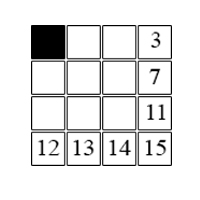
\includegraphics[width=0.30\textwidth]{fringe}
	\captionsetup{justification=centering}
	\caption{Fringe Database Pattern For Fifteen Tile}
\end{figure}

Once the breadth-first search has finished and it has trawled through all $518,914,400$ states, using IDA* the heuristic function determines the positions of the fringe tiles and the blank which are used as an index to the row with the given configuration in the database, the value for that row is then retrieved and used as the heuristic value.

\subsubsection{Non-Additive Pattern Database Limitations}
If the tiles are divided into disjoint groups, the best way to combine them admissibly is to take the maximum of their values; non-additive pattern database values include all moves needed to solve the configuration including moves of other tile. \citep{DBLP:journals/corr/abs-1107-0050}.

Another major issue is space required to store all possible states. When considering the 15 tile: provided each row in the database is 1 byte and there are 519,914,400 rows that's a total of 519Mb, and the time taken to perform the breadth-first search is extensive, Table1: Breadth-First Search Analysis shows that the time taken to expand just 65638 nodes was 34621.883ms.

Scalability is another issue regarding non-additive pattern databases. Take Figure 7 as an example, if we were to scale up to the twenty-five tile puzzle and performed the same calculations for taking the fringe: $25!/(25-10)!=1.1861676e+13$, provided each row in the database is 1 byte as previously stated, the summation is roughly 12 Terabytes worth of memory.



\begin{figure}[ht]
	\centering
	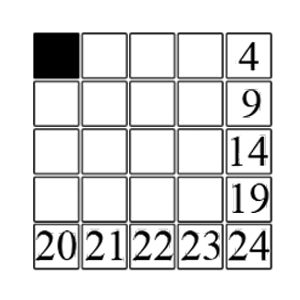
\includegraphics[width=0.35\textwidth]{fringe15}
	\captionsetup{justification=centering}
	\caption{Fringe Database Pattern For The Twenty-five Tile}
\end{figure}

\subsection{Statically-Partitioned Additive Database Heuristics}
In order to develop a statically-partitioned additive database for the sliding tile puzzle, I partitioned the tiles into disjoint groups, meaning each tile is placed in a group and only appears in that group. The same method as explained in 6.2 for finding all the states was computed for each subset; a breadth-first search from the goal state with all possible configurations of each tile in the disjoint groups and the number of moves required to get to the goal state. For a particular state in the search, for each position of the tiles an index was computed for the corresponding row in the database, then I retrieved the number of moves required to solve the tiles in that group and added this value to each value of the other disjoint groups. The summed total of these values will always be equal to or larger than the Manhattan distance of the state as it considers the interactions between tiles within a given subset.	

I initially chose to implement the 6-6-3 partitioning as I hypothesised it will be the best compromise between speed and memory in comparison with other possible solutions, Figure 8 shows the partitioning. The first two images display the fifteen tile with the subsets comprising of 6 tiles, $2\times(16!/(16-6)!)= 11531520$ states to be stored, the final subset requires $16!/(16-3)!=3360$ states stored that's a total of $11534880$ rows in the database. 


\begin{figure}[ht]
	\centering
	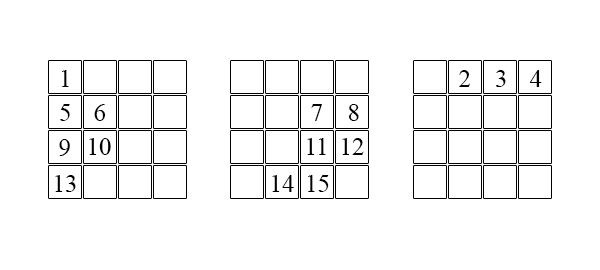
\includegraphics[width=0.9\textwidth]{15tile}
	\captionsetup{justification=centering}
	\caption{6-6-3 Partioning}
\end{figure}



\section{Gantt Chart}
	\begin{sideways}
		\newganttchartelement{voidbar}{
			voidbar/.style={
				draw=black,
				top color=black!25,
				bottom color=black!23
		}}
		\begin{ganttchart}[x unit=0.40cm, vgrid, title label font=\scriptsize,
			canvas/.style={draw=black, dotted}]{1}{23}
			\gantttitle{Project schedule shown for e-vision week numbers
				and semester week numbers}{23} \\
			\gantttitlelist{21,...,42}{1}\\
			\gantttitle{CB}{4}
			\gantttitlelist{1,...,10}{1}
			\gantttitle{EB}{4}
			\gantttitlelist{11,...,14}{1}\\
			
			
			%the elements, bars and milestones, are identified as elem0, elem1, etc
			
			%elem1
			\ganttbar{Sliding-tile implementation}{1}{4}     \\  %elem0  
			\ganttbar{Progress Report}{3}{5}    \\  %elem1 
			\ganttbar{Rubik's Cube Implementation}{5}{7}              \\  %elem2     
			\ganttbar{Additive Database Heuristic Cube }{8}{12}         \\
			\ganttbar{Evaluate Results}{10}{12}         \\
			\ganttbar{Experiments}{11}{13}  \\
	
			\ganttbar{Code delivery}{13}{22}                \\%elem3
			\ganttbar{Final report writing}{15}{22}                \\
			\ganttbar{Inspection preparation}{18}{22}                \\
			
			
			\ganttlink{elem0}{elem2}
		    \ganttlink{elem0}{elem1}
			\ganttlink{elem2}{elem3}
			\ganttlink{elem3}{elem4}
			\ganttlink{elem4}{elem5}
			\ganttlink{elem5}{elem6}
			\ganttlink{elem6}{elem7}
			\ganttlink{elem7}{elem8}

		\end{ganttchart}
	\end{sideways}


\clearpage
\bibliography{bibfile}


\appendix
\clearpage






\end{document}

